\documentclass[12pt, a4paper]{article}

\usepackage[utf8]{inputenc}
\usepackage{amsmath, amssymb}
\usepackage{graphicx}
\usepackage{hyperref}
\usepackage{geometry}
\usepackage{caption}
\usepackage{subcaption}
\usepackage{float}
\usepackage{booktabs}
\usepackage{enumitem}
\usepackage{xcolor}
\usepackage{listings}

\geometry{margin=1in}
\graphicspath{{plots/}}

\hypersetup{
    colorlinks=true,
    linkcolor=blue,
    urlcolor=blue,
    citecolor=blue
}

\lstset{
    basicstyle=\ttfamily\small,
    breaklines=true,
    frame=single,
    language=Python,
    keywordstyle=\color{blue},
    commentstyle=\color{gray}
}

\title{\textbf{Risk-Aware Hybrid LQR-MPC Navigation\\for Autonomous Systems}\\[0.5em]\large Implementation and Evaluation Report}
\author{Kshitiz Kumar Sinha \and Agolika BM}
\date{\today}

\begin{document}

\maketitle

\begin{abstract}
This report documents the complete design, implementation, testing, and debugging of a Risk-Aware Hybrid LQR-MPC navigation framework for a differential-drive mobile robot. The system combines the computational efficiency of a Linear Quadratic Regulator (LQR) with the constraint-handling capability of Model Predictive Control (MPC) through a continuous sigmoid-based blending supervisor. We implemented four distinct controller variants: pure LQR for baseline tracking, a CVXPY-based Tube MPC with obstacle avoidance, a CasADi-based Adaptive Nonlinear MPC with online parameter estimation, and a Hybrid LQR-MPC blended controller. This report honestly presents what worked, what failed, and how we debugged each issue. The framework was validated both in offline Python simulations and in a ROS2 Jazzy Gazebo environment using a Turtlebot3 Burger.
\end{abstract}

\vspace{0.3cm}
\noindent\textbf{GitHub Repository:} \url{https://github.com/Erebuzzz/Risk-Aware-Hybrid-LQR-MPC-Navigation-for-Autonomous-Systems}

\tableofcontents
\newpage

%% ============================================================
\section{Introduction}
%% ============================================================

Autonomous navigation in obstacle-dense environments requires controllers that can simultaneously track a desired trajectory and react to nearby hazards. A pure LQR controller is computationally cheap and provides excellent tracking in open space, but it has no mechanism to handle state constraints such as obstacle avoidance. Conversely, an MPC controller can naturally encode obstacle constraints, but solving the optimization problem at high frequency is computationally expensive.

Our project addresses this trade-off by designing a \textbf{hybrid architecture} that runs LQR as the default high-frequency tracker and smoothly blends in MPC only when the robot's risk level rises due to obstacle proximity. The blending weight $w(t) \in [0,1]$ is computed from a sigmoid-based risk function with hysteresis and rate limiting to prevent chattering.

\subsection{Project Goals}
\begin{enumerate}
    \item Implement a discrete-time LQR controller for trajectory tracking on a differential-drive robot.
    \item Implement a Tube MPC controller with linearized obstacle avoidance constraints using CVXPY.
    \item Implement an Adaptive Nonlinear MPC using CasADi with online LMS parameter estimation.
    \item Design and implement a hybrid blending supervisor that continuously arbitrates between LQR and MPC.
    \item Validate all controllers in both offline simulation and a ROS2 Gazebo environment.
\end{enumerate}

\subsection{Robot Model}
We use a standard unicycle (differential-drive) kinematic model:
\begin{align}
    \dot{x} &= v \cos\theta \label{eq:dyn_x}\\
    \dot{y} &= v \sin\theta \label{eq:dyn_y}\\
    \dot{\theta} &= \omega \label{eq:dyn_theta}
\end{align}
where $(x, y)$ is the robot's position, $\theta$ is the heading, $v$ is the linear velocity, and $\omega$ is the angular velocity. The control input is $\mathbf{u} = [v, \omega]^T$, subject to actuator bounds $|v| \leq v_{\max}$ and $|\omega| \leq \omega_{\max}$.


%% ============================================================
\section{LQR Controller}
%% ============================================================

\subsection{Formulation}
The LQR controller linearizes the nonlinear dynamics around a time-varying reference trajectory $(\mathbf{x}_r(t), \mathbf{u}_r(t))$. Defining the tracking error $\tilde{\mathbf{x}}_k = \mathbf{x}_k - \mathbf{x}_{r,k}$, the linearized discrete-time system is:
\begin{equation}
    \tilde{\mathbf{x}}_{k+1} = A_d \tilde{\mathbf{x}}_k + B_d \tilde{\mathbf{u}}_k
\end{equation}
where $A_d$ and $B_d$ are obtained by Jacobian linearization at the current operating point $(v_r, \theta_r)$ and discretized with sampling time $\Delta t$.

The optimal feedback gain $K$ is computed by solving the Discrete Algebraic Riccati Equation (DARE):
\begin{equation}
    P = A_d^T P A_d - A_d^T P B_d (R + B_d^T P B_d)^{-1} B_d^T P A_d + Q
\end{equation}
\begin{equation}
    K = (R + B_d^T P B_d)^{-1} B_d^T P A_d
\end{equation}

The control law is:
\begin{equation}
    \mathbf{u}_k = \mathbf{u}_{r,k} - K \tilde{\mathbf{x}}_k
\end{equation}

\subsection{Implementation Details}
\begin{itemize}
    \item \textbf{Weight matrices:} $Q = \text{diag}(10, 10, 1)$, $R = \text{diag}(0.1, 0.1)$. The higher weight on position errors ensures tight spatial tracking, while the lower heading weight allows smoother turning.
    \item \textbf{DARE fallback chain:} If the DARE solver fails at a given operating point (e.g., near $v_r = 0$ where controllability is lost), we implemented a three-level fallback: (1) use the last successfully cached gain, (2) solve DARE at a nominal point $(v=0.1, \theta=0)$, (3) fall back to a conservative proportional gain.
    \item \textbf{Angle wrapping:} Heading error is normalized to $[-\pi, \pi]$ to prevent discontinuities.
\end{itemize}

\subsection{LQR Results}
The LQR controller was tested on a figure-8 trajectory in an obstacle-free environment. It achieved a mean tracking error of \textbf{0.005 m} with a final error of \textbf{0.003 m}, demonstrating sub-centimeter accuracy.

\begin{figure}[H]
    \centering
    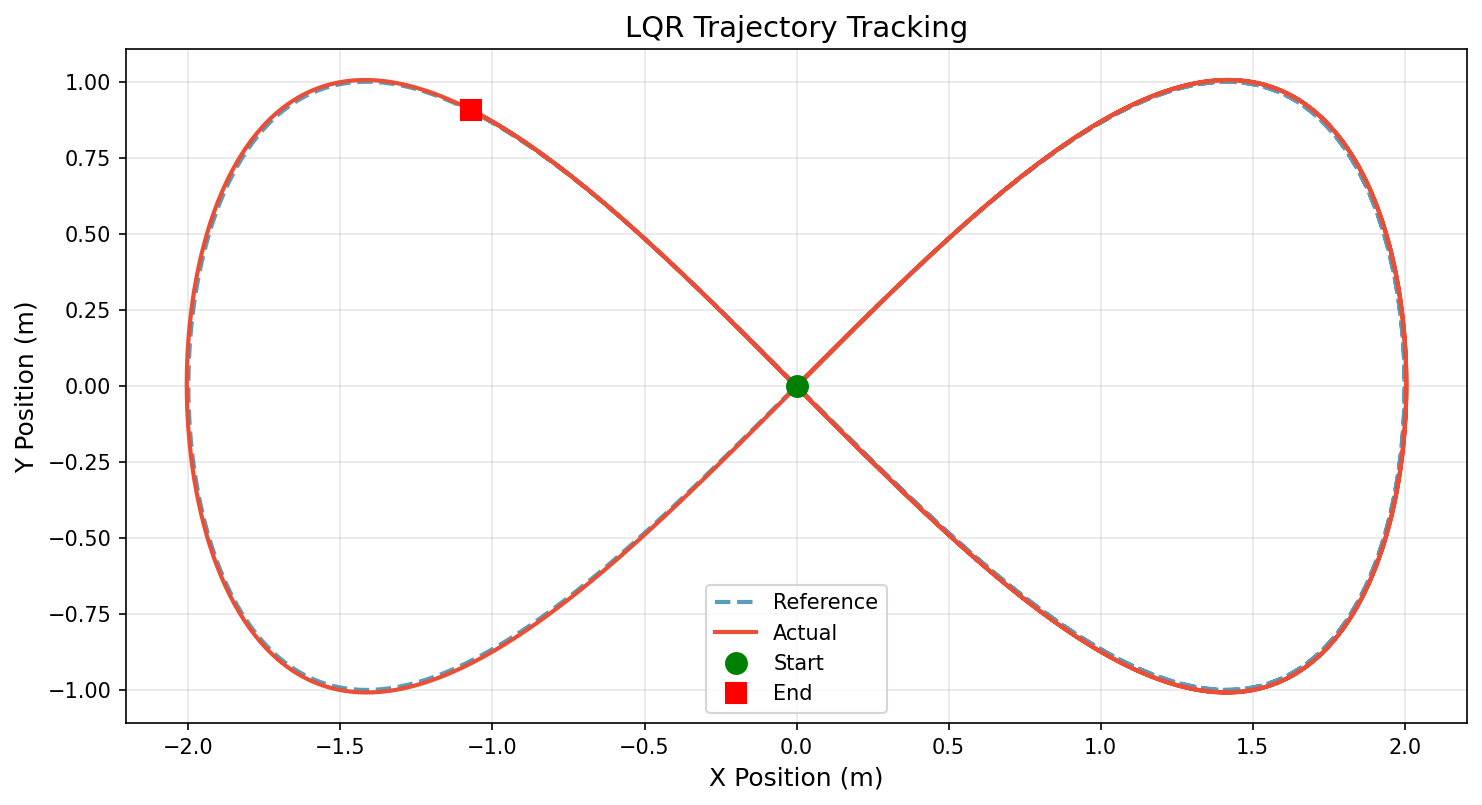
\includegraphics[width=0.85\textwidth]{lqr_tracking.png}
    \caption{LQR trajectory tracking on a figure-8 path. The robot (blue) closely follows the reference (dashed red) with sub-centimeter accuracy.}
    \label{fig:lqr_tracking}
\end{figure}

\begin{figure}[H]
    \centering
    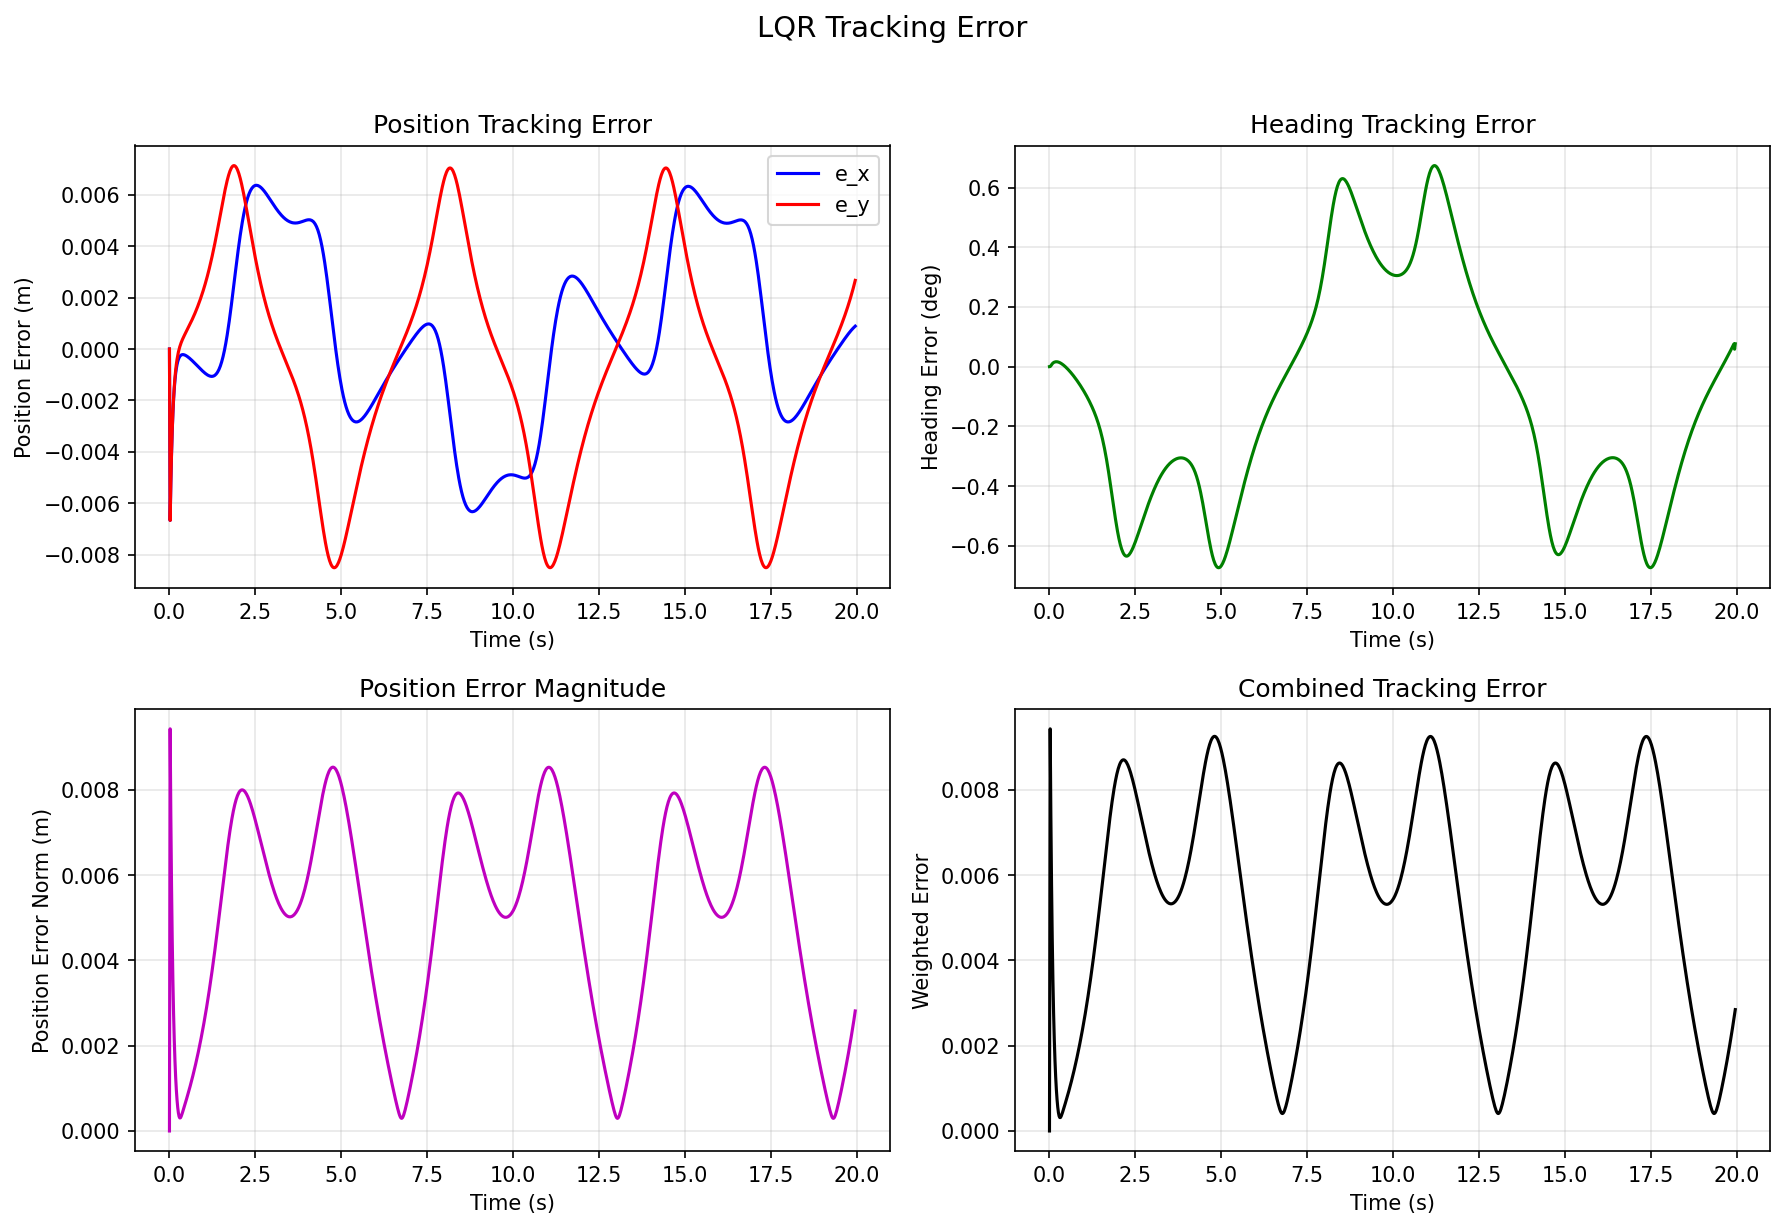
\includegraphics[width=0.85\textwidth]{lqr_error.png}
    \caption{LQR tracking error over time. The error remains bounded below 0.015 m throughout the 20-second simulation.}
    \label{fig:lqr_error}
\end{figure}

\begin{figure}[H]
    \centering
    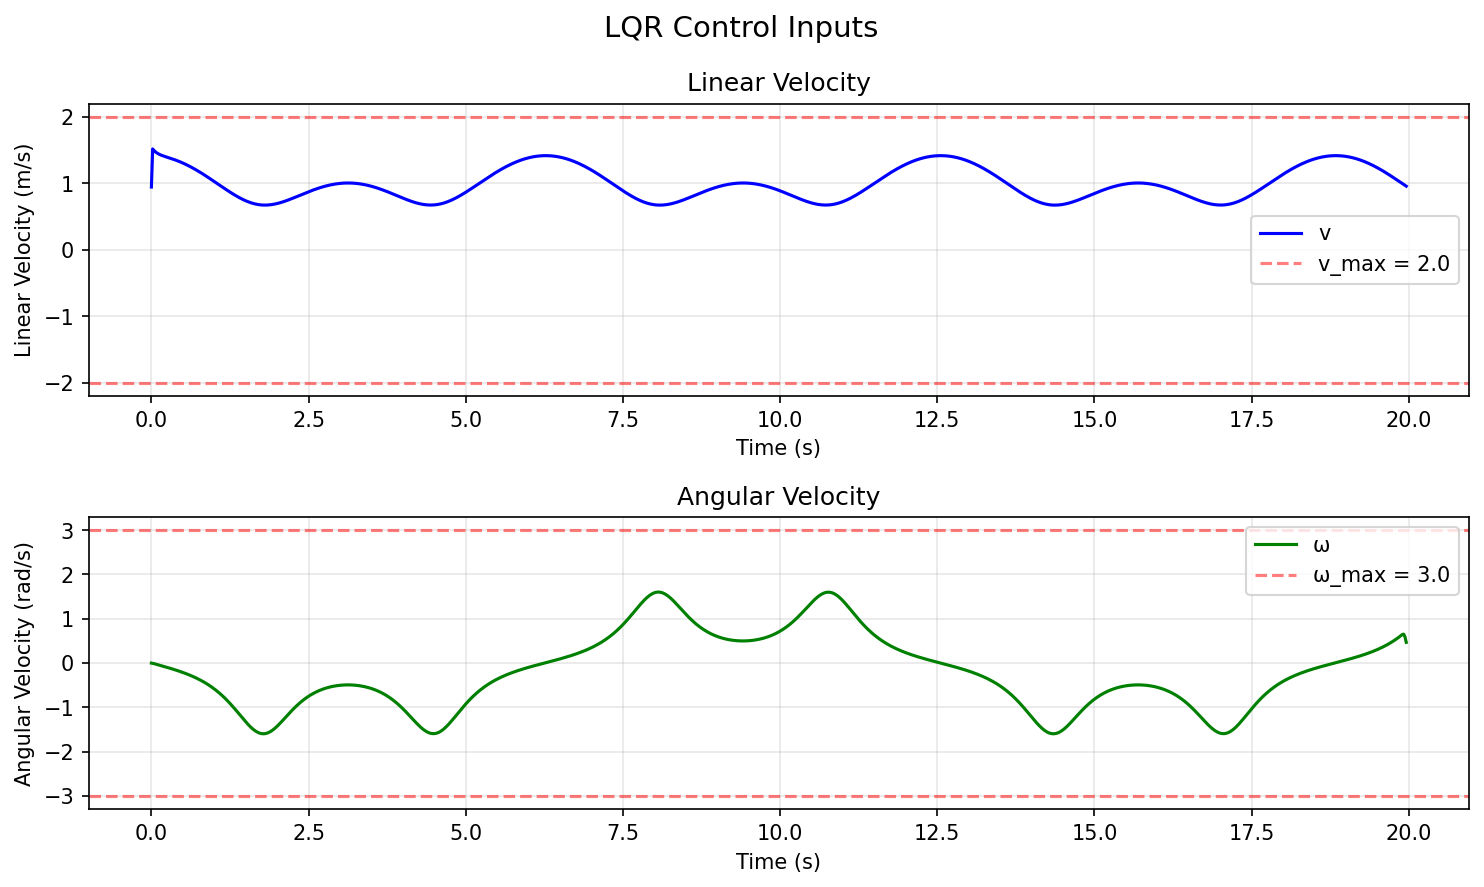
\includegraphics[width=0.85\textwidth]{lqr_control.png}
    \caption{LQR control inputs ($v$ and $\omega$) over time, showing smooth actuator commands within bounds.}
    \label{fig:lqr_control}
\end{figure}


%% ============================================================
\section{MPC Controller (Tube MPC)}
%% ============================================================

\subsection{Formulation}
The MPC controller solves a finite-horizon optimization problem at each timestep using CVXPY with the OSQP solver:
\begin{equation}
    \min_{\mathbf{u}_{0:N-1}} \sum_{k=0}^{N-1} \left( \|\mathbf{x}_k - \mathbf{x}_{r,k}\|_Q^2 + \|\mathbf{u}_k - \mathbf{u}_{r,k}\|_R^2 \right) + \|\mathbf{x}_N - \mathbf{x}_{r,N}\|_P^2
\end{equation}
subject to:
\begin{align}
    \mathbf{x}_{k+1} &= A_d \mathbf{x}_k + B_d \mathbf{u}_k & \text{(linearized dynamics)} \\
    |v_k| &\leq v_{\max},\quad |\omega_k| \leq \omega_{\max} & \text{(actuator limits)} \\
    \|\mathbf{p}_k - \mathbf{p}_{\text{obs}}\| &\geq d_{\text{safe}} & \text{(obstacle avoidance)}
\end{align}

The terminal cost matrix $P$ is computed as the solution to the DARE, providing an implicit infinite-horizon tail cost.

\subsection{Obstacle Avoidance}
The nonlinear Euclidean distance constraint is linearized around the current predicted position using a first-order Taylor expansion. To handle infeasibility when obstacles are too close, we introduce slack variables $\xi_k$ with a high penalty $\rho = 5000$:
\begin{equation}
    \|\mathbf{p}_k - \mathbf{p}_{\text{obs}}\| \geq d_{\text{safe}} - \xi_k, \quad \xi_k \geq 0
\end{equation}

\subsection{MPC Results}
The MPC was tested on a figure-8 trajectory with 3 circular obstacles. It achieved a mean tracking error of \textbf{1.638 m} with a mean solve time of \textbf{163 ms}. The higher error compared to LQR is expected since the controller must deviate from the reference to avoid obstacles. However, we observed \textbf{163 collision events} where the robot's distance to an obstacle fell below $d_{\text{safe}}$, indicating that the linearized constraint approximation is sometimes too conservative or too loose depending on the geometry.

\begin{figure}[H]
    \centering
    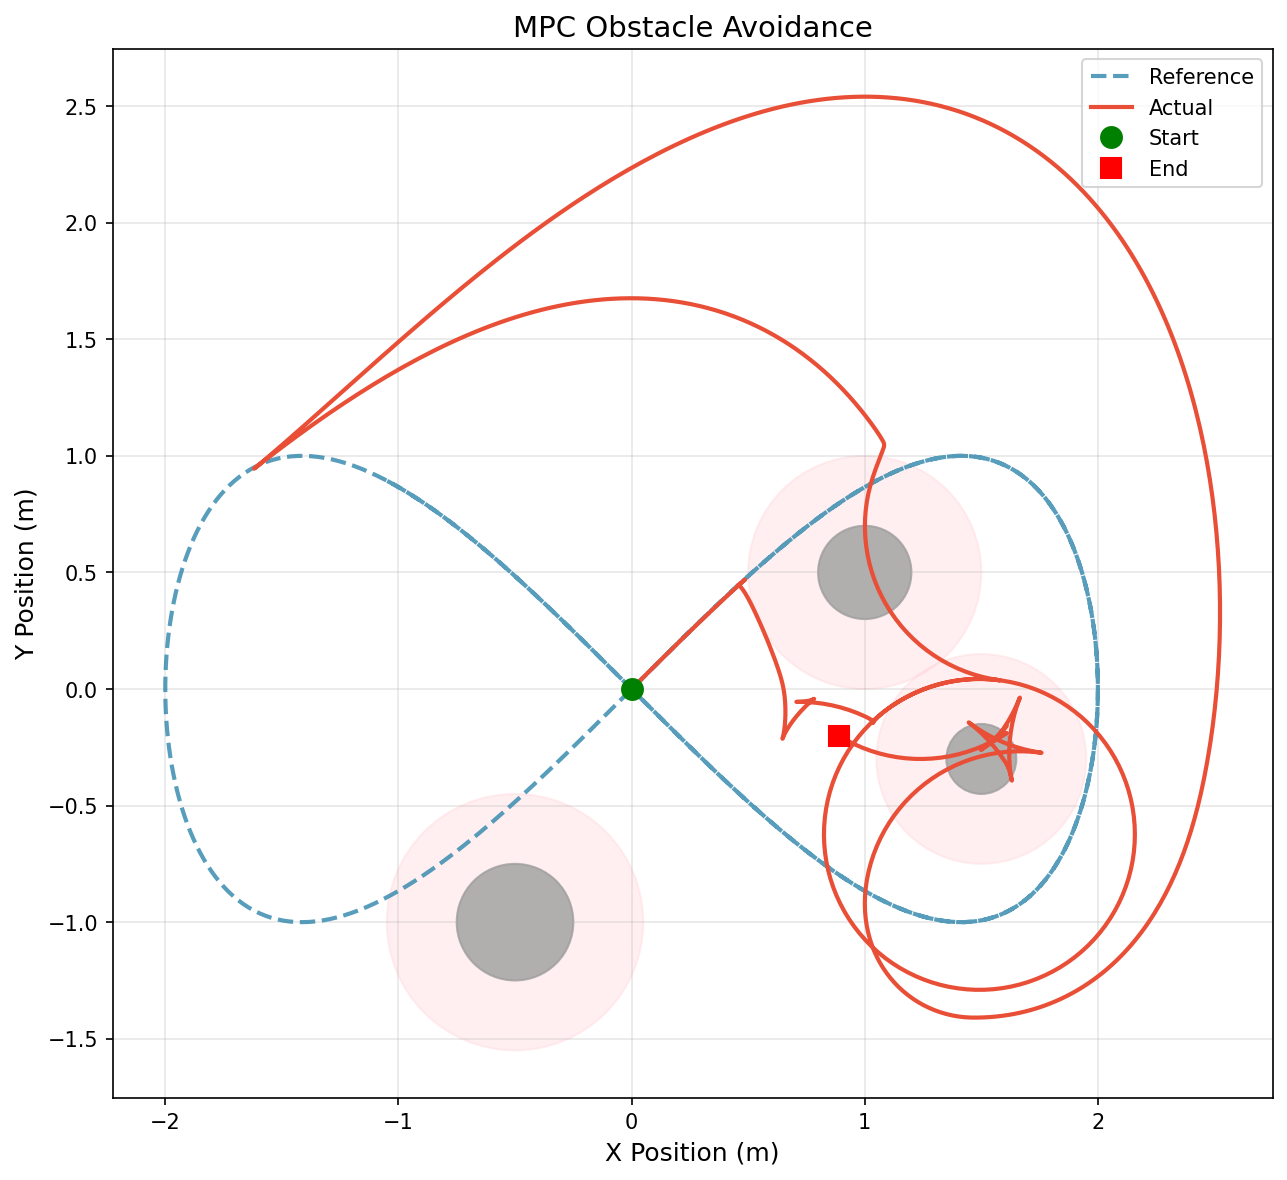
\includegraphics[width=0.85\textwidth]{mpc_obstacle_avoidance.png}
    \caption{MPC trajectory with obstacle avoidance. The robot deviates from the reference path to navigate around circular obstacles (shown as red circles with safety margins).}
    \label{fig:mpc_traj}
\end{figure}

\begin{figure}[H]
    \centering
    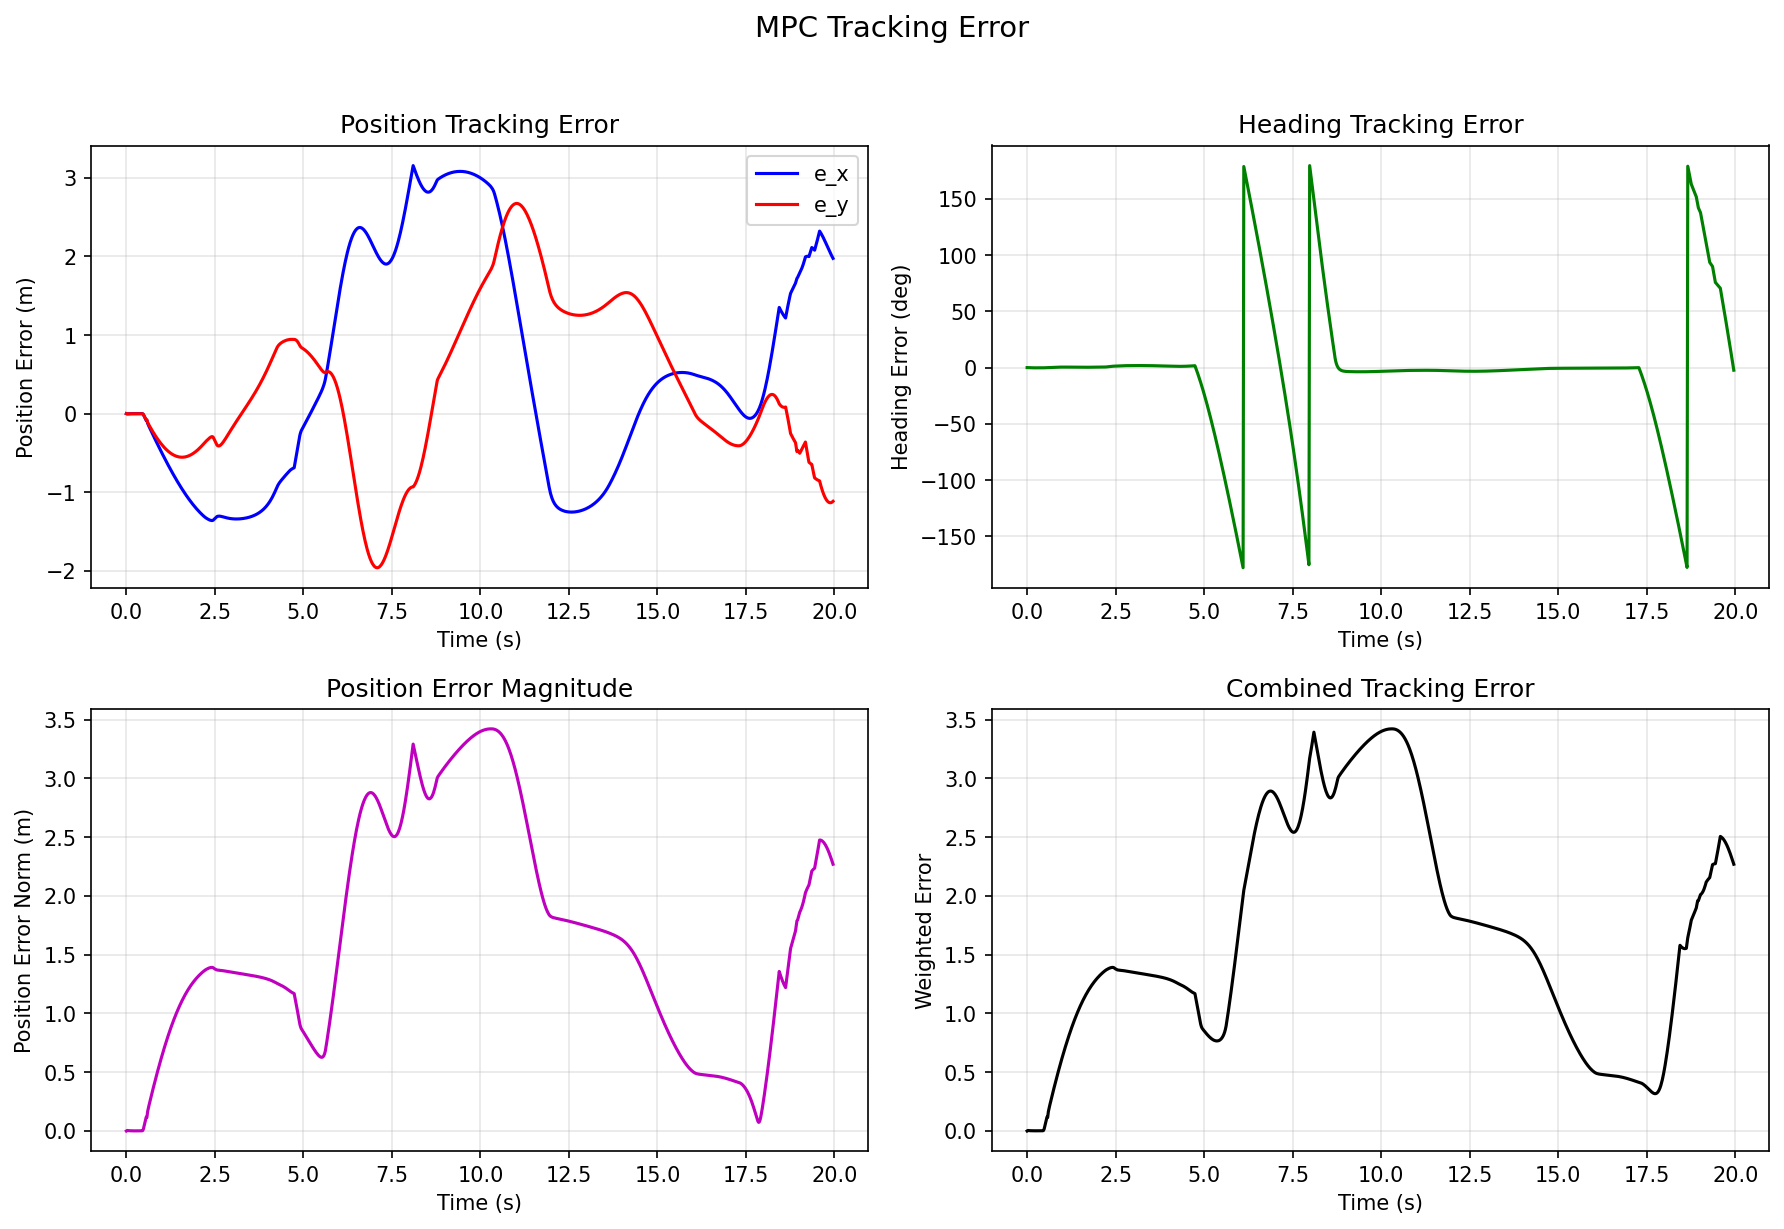
\includegraphics[width=0.85\textwidth]{mpc_error.png}
    \caption{MPC tracking error over time, showing spikes when the robot diverts around obstacles.}
    \label{fig:mpc_error}
\end{figure}

\begin{figure}[H]
    \centering
    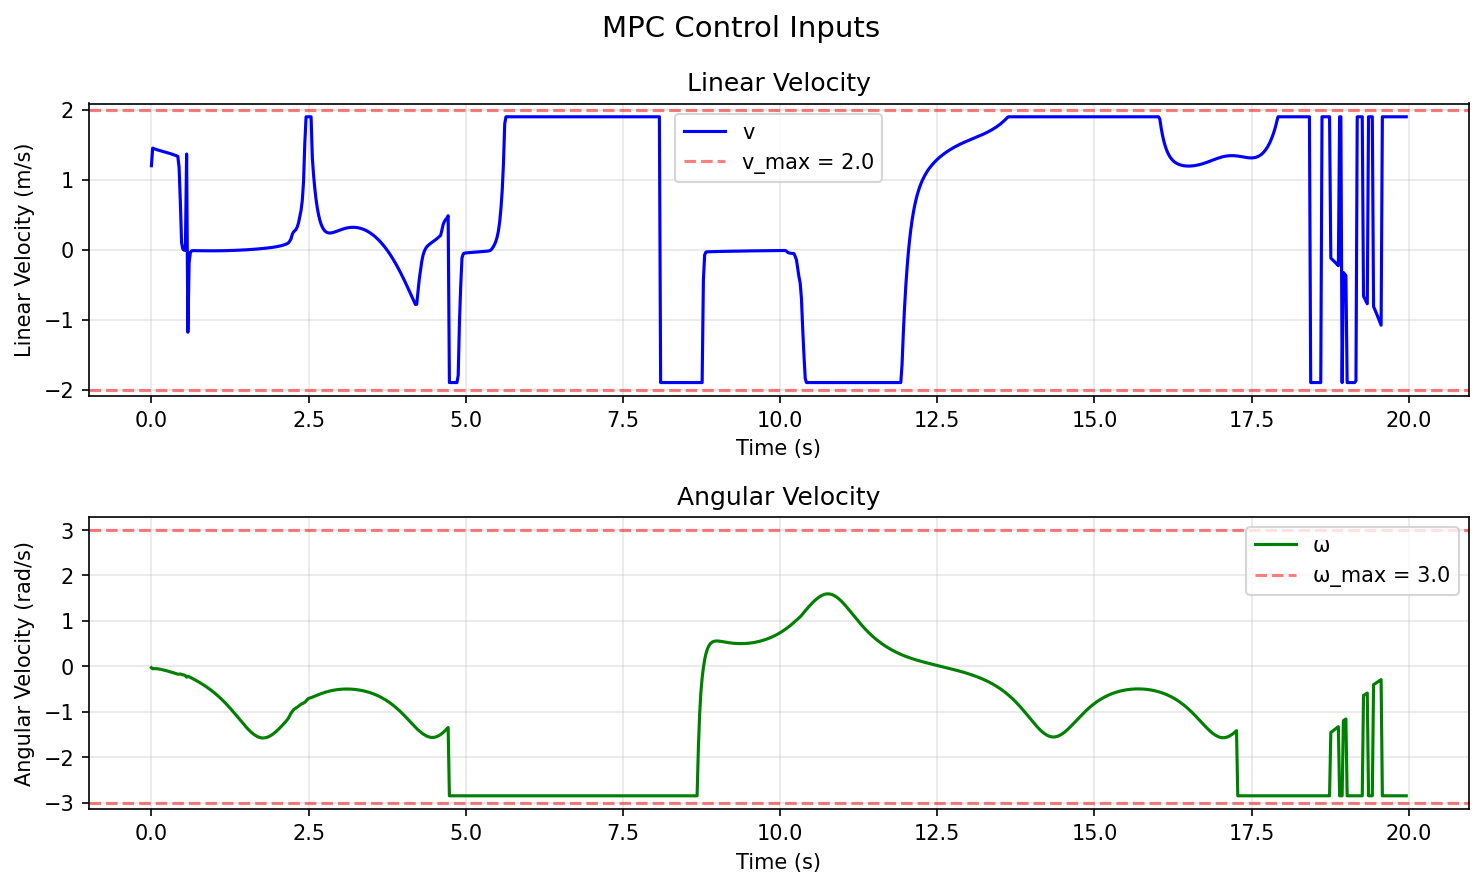
\includegraphics[width=0.85\textwidth]{mpc_control.png}
    \caption{MPC control inputs showing the solver's response to obstacle proximity.}
    \label{fig:mpc_control}
\end{figure}


%% ============================================================
\section{Adaptive Nonlinear MPC (CasADi)}
%% ============================================================

\subsection{Formulation}
The Adaptive NMPC uses CasADi with the IPOPT solver to solve the \emph{exact} nonlinear dynamics (no linearization), providing better constraint satisfaction in tight spaces:
\begin{equation}
    \min \sum_{k=0}^{N-1} \left( \|\mathbf{x}_k - \mathbf{x}_{r,k}\|_Q^2 + \|\mathbf{u}_k - \mathbf{u}_{r,k}\|_R^2 + q_\xi \|\xi_k\|^2 \right) + \omega_T \sum_{k=N}^{N+M} (\cdots)
\end{equation}
subject to the full nonlinear dynamics $\mathbf{x}_{k+1} = f(\mathbf{x}_k, \mathbf{u}_k)$ and exact Euclidean obstacle constraints.

\subsection{Extended Terminal Horizon}
Beyond the prediction horizon $N$, we roll out $M$ additional steps using a pre-computed LQR feedback policy $\mathbf{u}_k = \mathbf{u}_{r,k} - K(\mathbf{x}_k - \mathbf{x}_{r,k})$. This provides a stabilizing terminal controller that improves closed-loop performance without increasing the number of free optimization variables.

\subsection{Online Parameter Adaptation (LMS)}
The Adaptive MPC includes an LMS filter that estimates unknown friction/slip parameters $\hat{\theta} = [\hat{\theta}_v, \hat{\theta}_\omega]^T$ online. The adapted dynamics become:
\begin{align}
    \dot{x} &= \hat{\theta}_v \cdot v \cos\theta \\
    \dot{y} &= \hat{\theta}_v \cdot v \sin\theta \\
    \dot{\theta} &= \hat{\theta}_\omega \cdot \omega
\end{align}
The LMS update rule is:
\begin{equation}
    \hat{\theta}_{k+1} = \hat{\theta}_k + \Gamma \Phi_k^T (\mathbf{x}_{\text{measured}} - \mathbf{x}_{\text{predicted}})
\end{equation}
where $\Gamma = 0.005 \cdot I$ is the adaptation gain and $\Phi_k$ is the regressor matrix.

\subsection{Adaptive MPC Results}
The Adaptive NMPC achieved a mean tracking error of \textbf{1.282 m} (better than the linearized MPC's 1.638 m) with a mean solve time of \textbf{145 ms}. However, it recorded \textbf{355 collision events}, more than the Tube MPC. This is because the nonlinear solver explores more aggressive paths that cut closer to obstacles.

\begin{figure}[H]
    \centering
    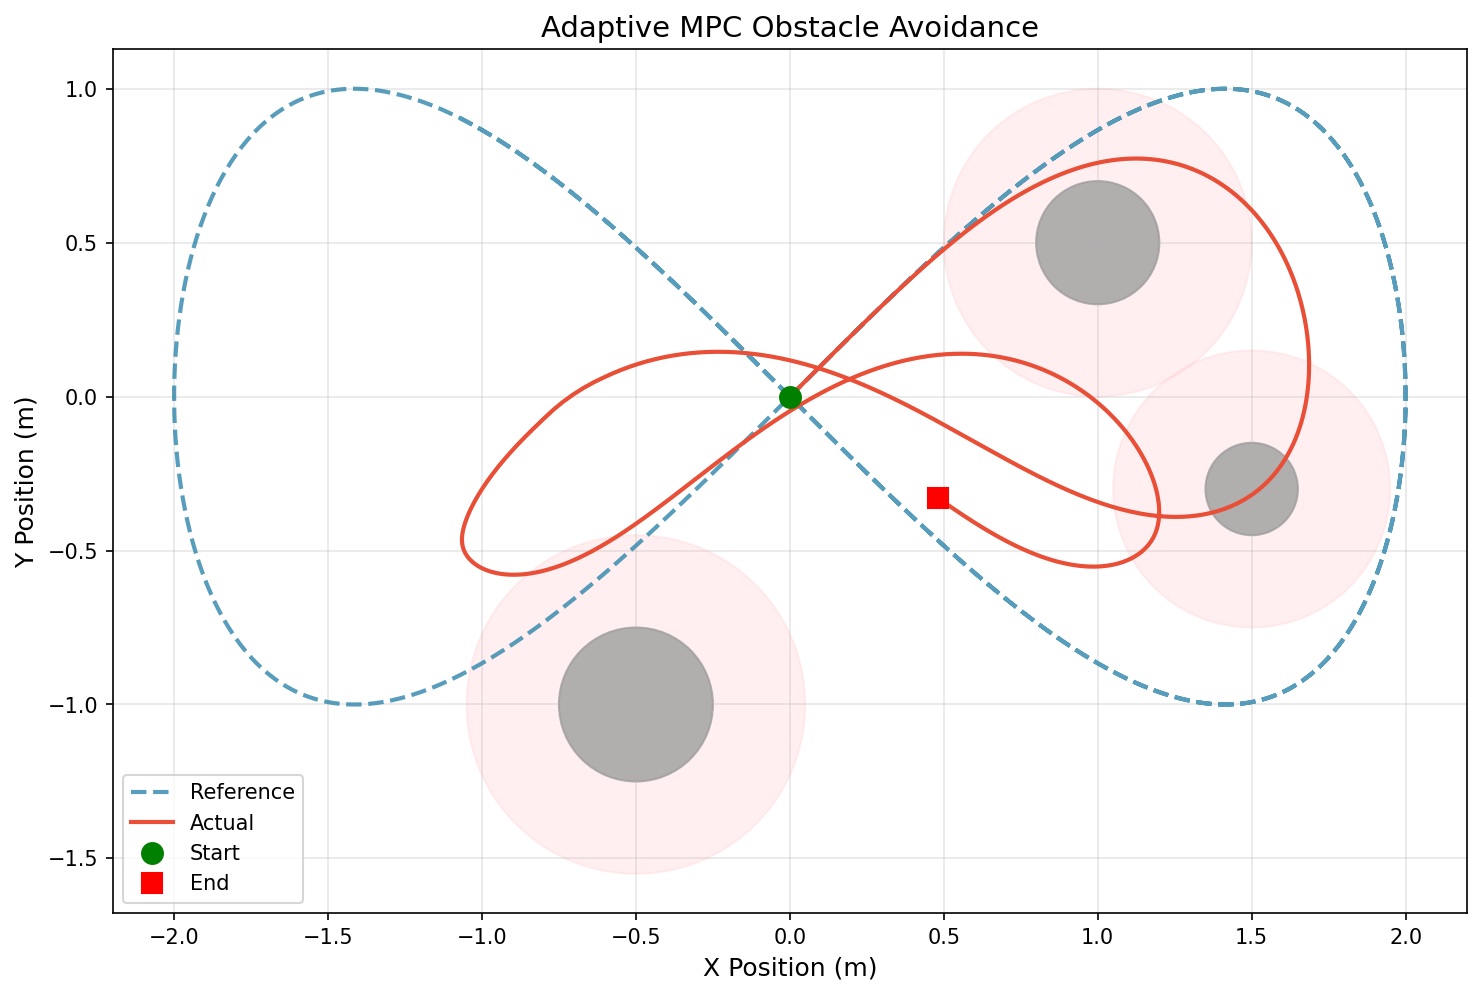
\includegraphics[width=0.85\textwidth]{adaptive_mpc_obstacle_avoidance.png}
    \caption{Adaptive NMPC trajectory with obstacle avoidance. The nonlinear solver finds tighter paths around obstacles compared to the linearized MPC.}
    \label{fig:ampc_traj}
\end{figure}

\begin{figure}[H]
    \centering
    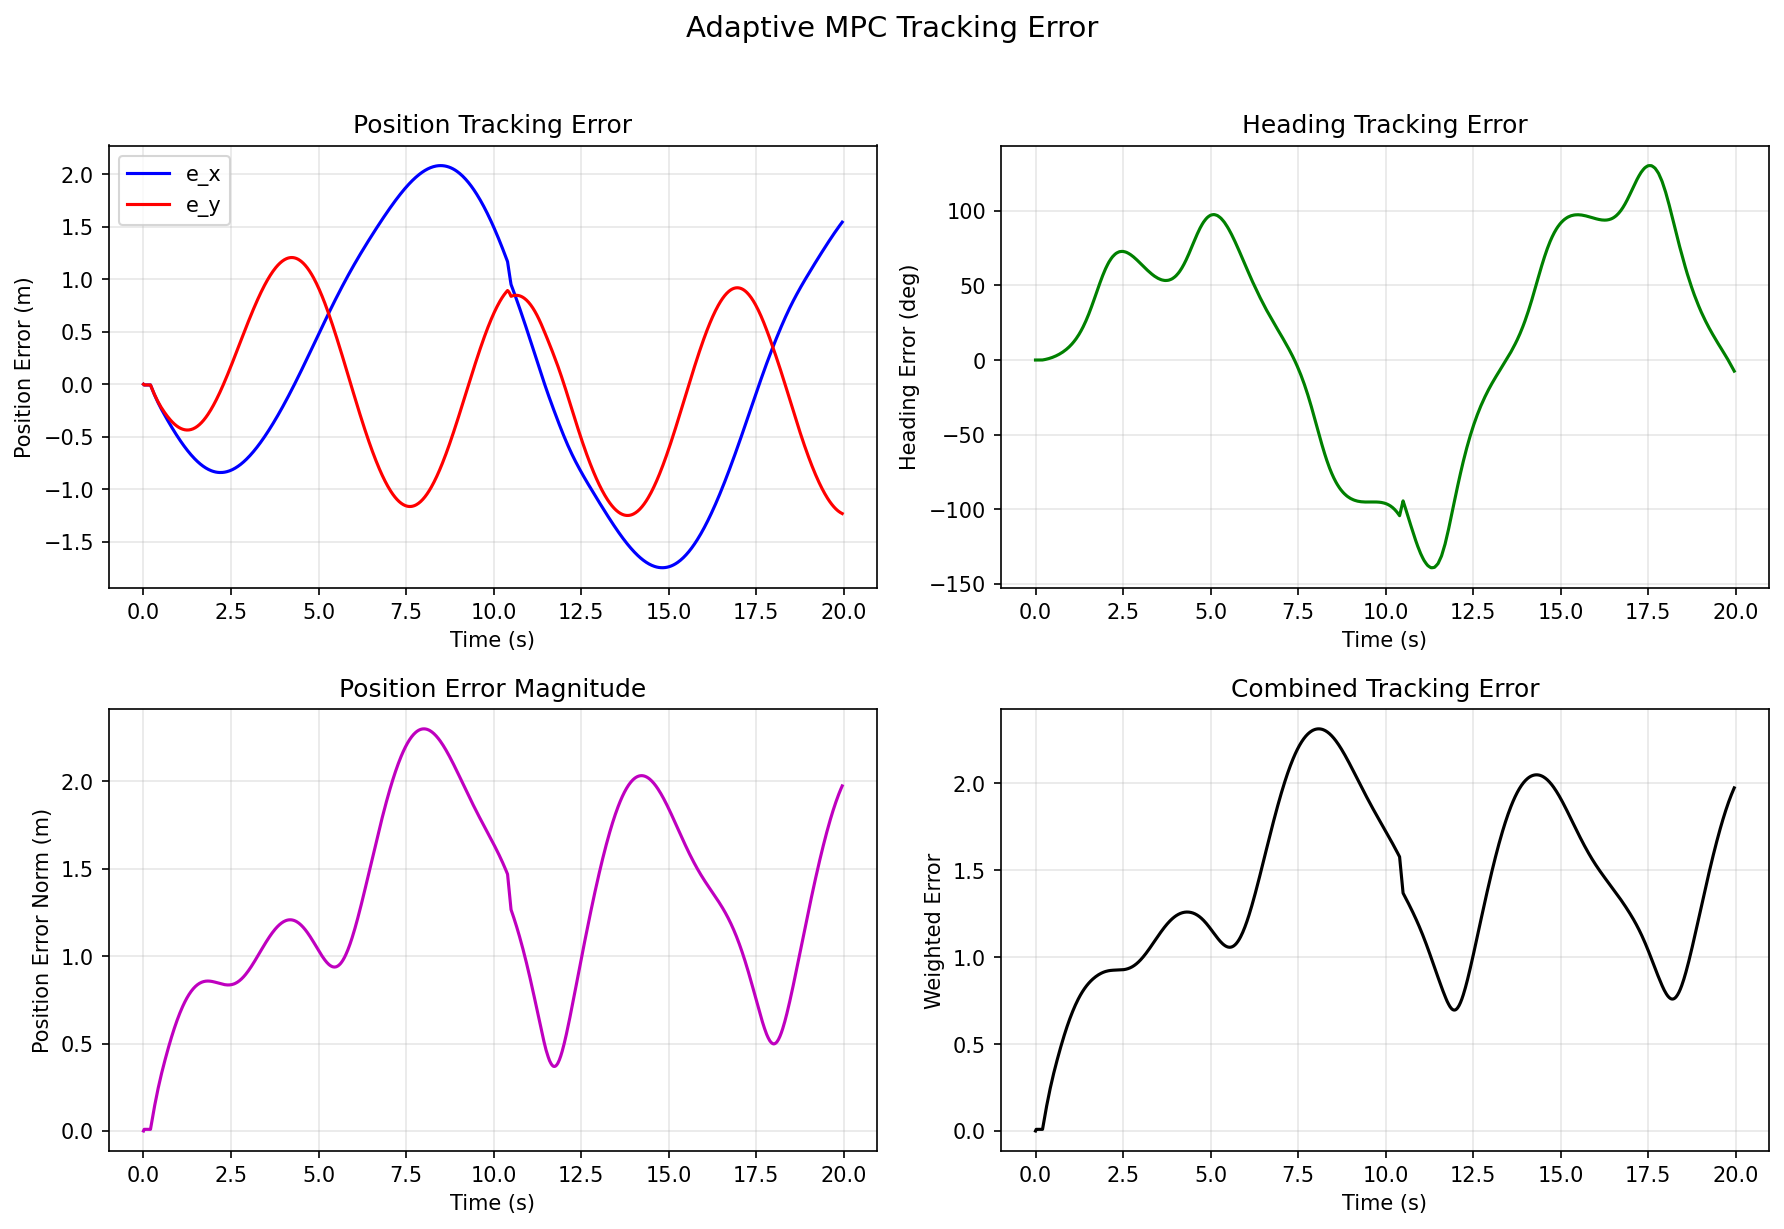
\includegraphics[width=0.85\textwidth]{adaptive_mpc_error.png}
    \caption{Adaptive NMPC tracking error over time.}
    \label{fig:ampc_error}
\end{figure}

\begin{figure}[H]
    \centering
    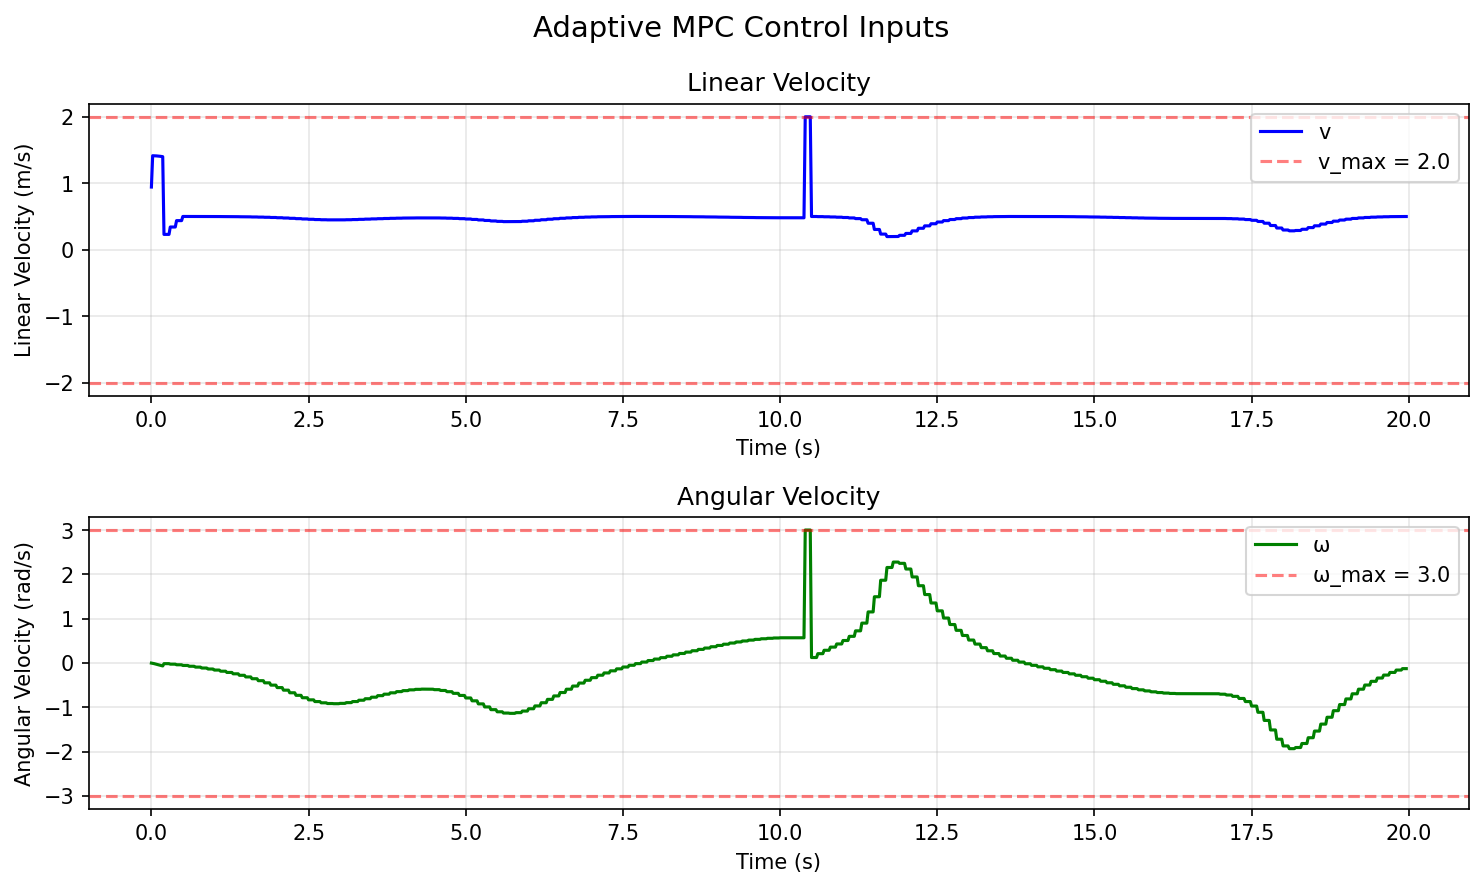
\includegraphics[width=0.85\textwidth]{adaptive_mpc_control.png}
    \caption{Adaptive NMPC control inputs.}
    \label{fig:ampc_control}
\end{figure}


%% ============================================================
\section{Hybrid LQR-MPC Controller}
%% ============================================================

\subsection{Blending Architecture}
The core contribution of this project is the Hybrid controller, which continuously blends LQR and MPC outputs:
\begin{equation}
    \mathbf{u}_{\text{blend}} = w(t) \cdot \mathbf{u}_{\text{MPC}} + (1 - w(t)) \cdot \mathbf{u}_{\text{LQR}}
\end{equation}
where $w(t) \in [0, 1]$ is computed through a four-stage pipeline:

\begin{enumerate}
    \item \textbf{Risk Assessment:} A combined risk metric $r \in [0,1]$ is computed from distance-based obstacle proximity ($\alpha = 0.6$) and predictive trajectory risk ($\beta = 0.4$).
    \item \textbf{Sigmoid Mapping:} $w_{\text{raw}} = \sigma(k \cdot (r - r_{\text{threshold}}))$ with steepness $k = 8$.
    \item \textbf{Hysteresis Deadband:} When $|r - r_{\text{threshold}}| < 0.08$, the weight is held constant to prevent oscillatory switching.
    \item \textbf{Asymmetric Rate Limiting:} Fast attack ($dw/dt \leq 20$/s when risk increases) and slow decay ($dw/dt \leq 2$/s when risk decreases) ensure rapid obstacle response but smooth path re-acquisition.
\end{enumerate}

\subsection{Anti-Chatter Guarantees}
The rate-limited weight $w(t)$ is Lipschitz-continuous with constant $L = dw_{\max}$. This guarantees:
\begin{itemize}
    \item Maximum weight change per timestep: $dw_{\max} \cdot \Delta t$
    \item Minimum time for full LQR$\to$MPC transition: $1/dw_{\max}$ seconds
    \item The blended output $\mathbf{u}_{\text{blend}}$ preserves actuator bounds by convexity if both $\mathbf{u}_{\text{LQR}}$ and $\mathbf{u}_{\text{MPC}}$ satisfy them individually.
\end{itemize}

\subsection{Hybrid Results}
The Hybrid controller achieved the best overall results among the obstacle-aware controllers:
\begin{itemize}
    \item Mean tracking error: \textbf{0.218 m} (vs.\ 1.638 m for MPC, 1.282 m for AMPC)
    \item Final tracking error: \textbf{0.056 m}
    \item Mean MPC solve time: \textbf{101.87 ms}
    \item MPC-dominant mode: 84.7\% of the time, Blended: 15.3\%
\end{itemize}

The significantly lower tracking error is because the blending supervisor uses MPC only for obstacle avoidance and allows LQR to maintain precise tracking in safe regions.

\begin{figure}[H]
    \centering
    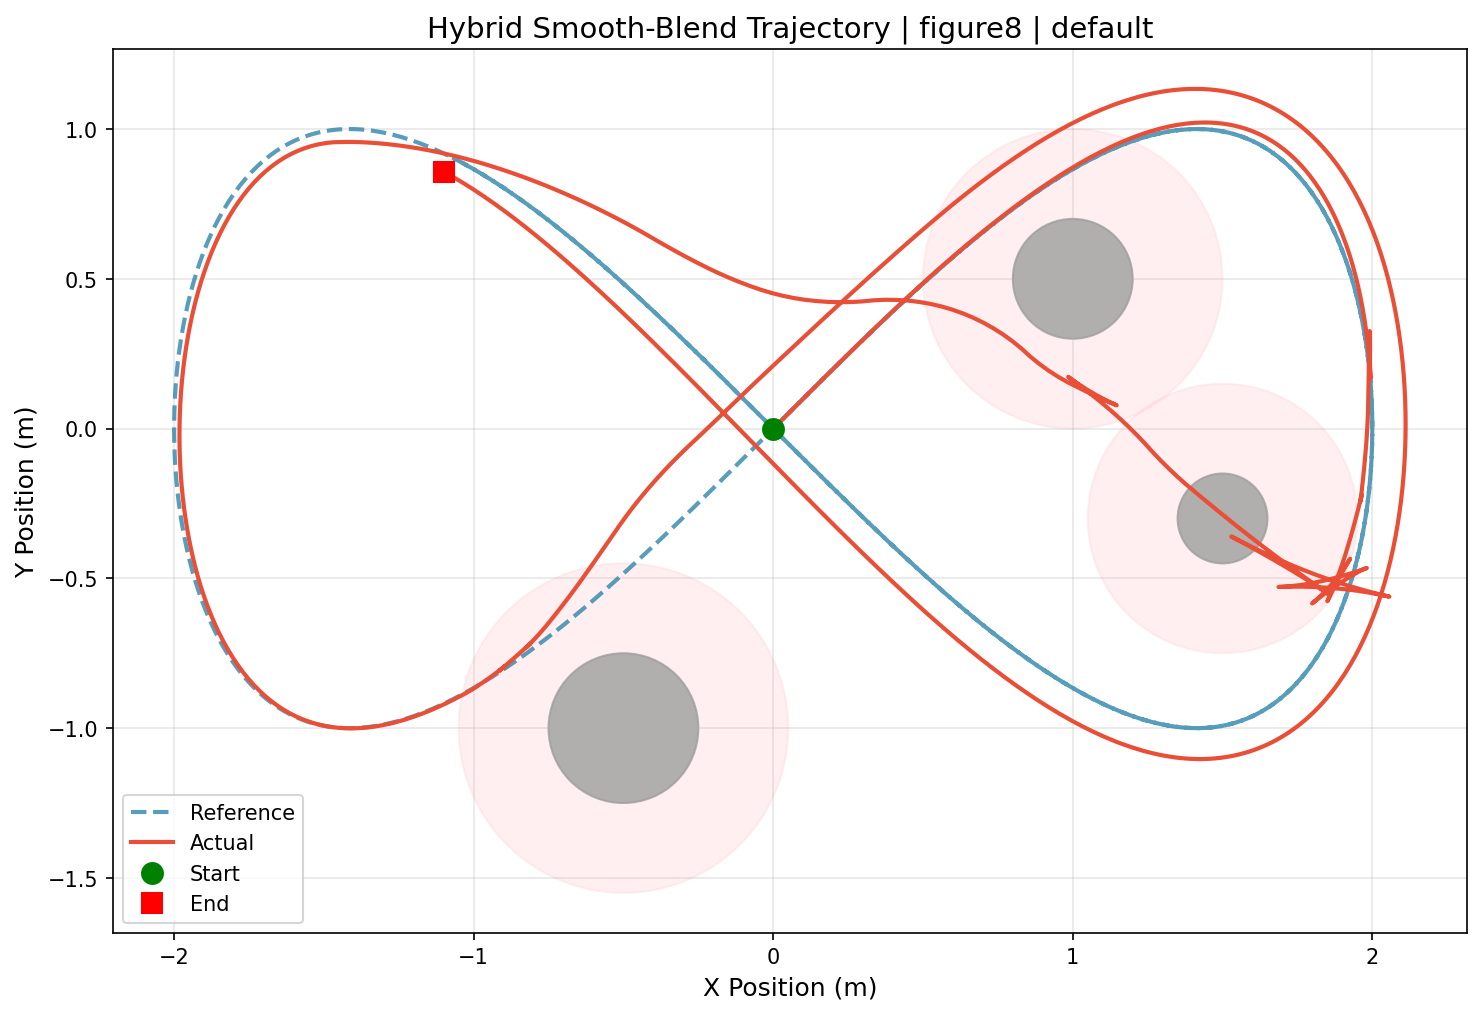
\includegraphics[width=0.85\textwidth]{hybrid_figure8_default_trajectory.png}
    \caption{Hybrid LQR-MPC trajectory showing smooth obstacle avoidance with tight path re-acquisition.}
    \label{fig:hybrid_traj}
\end{figure}

\begin{figure}[H]
    \centering
    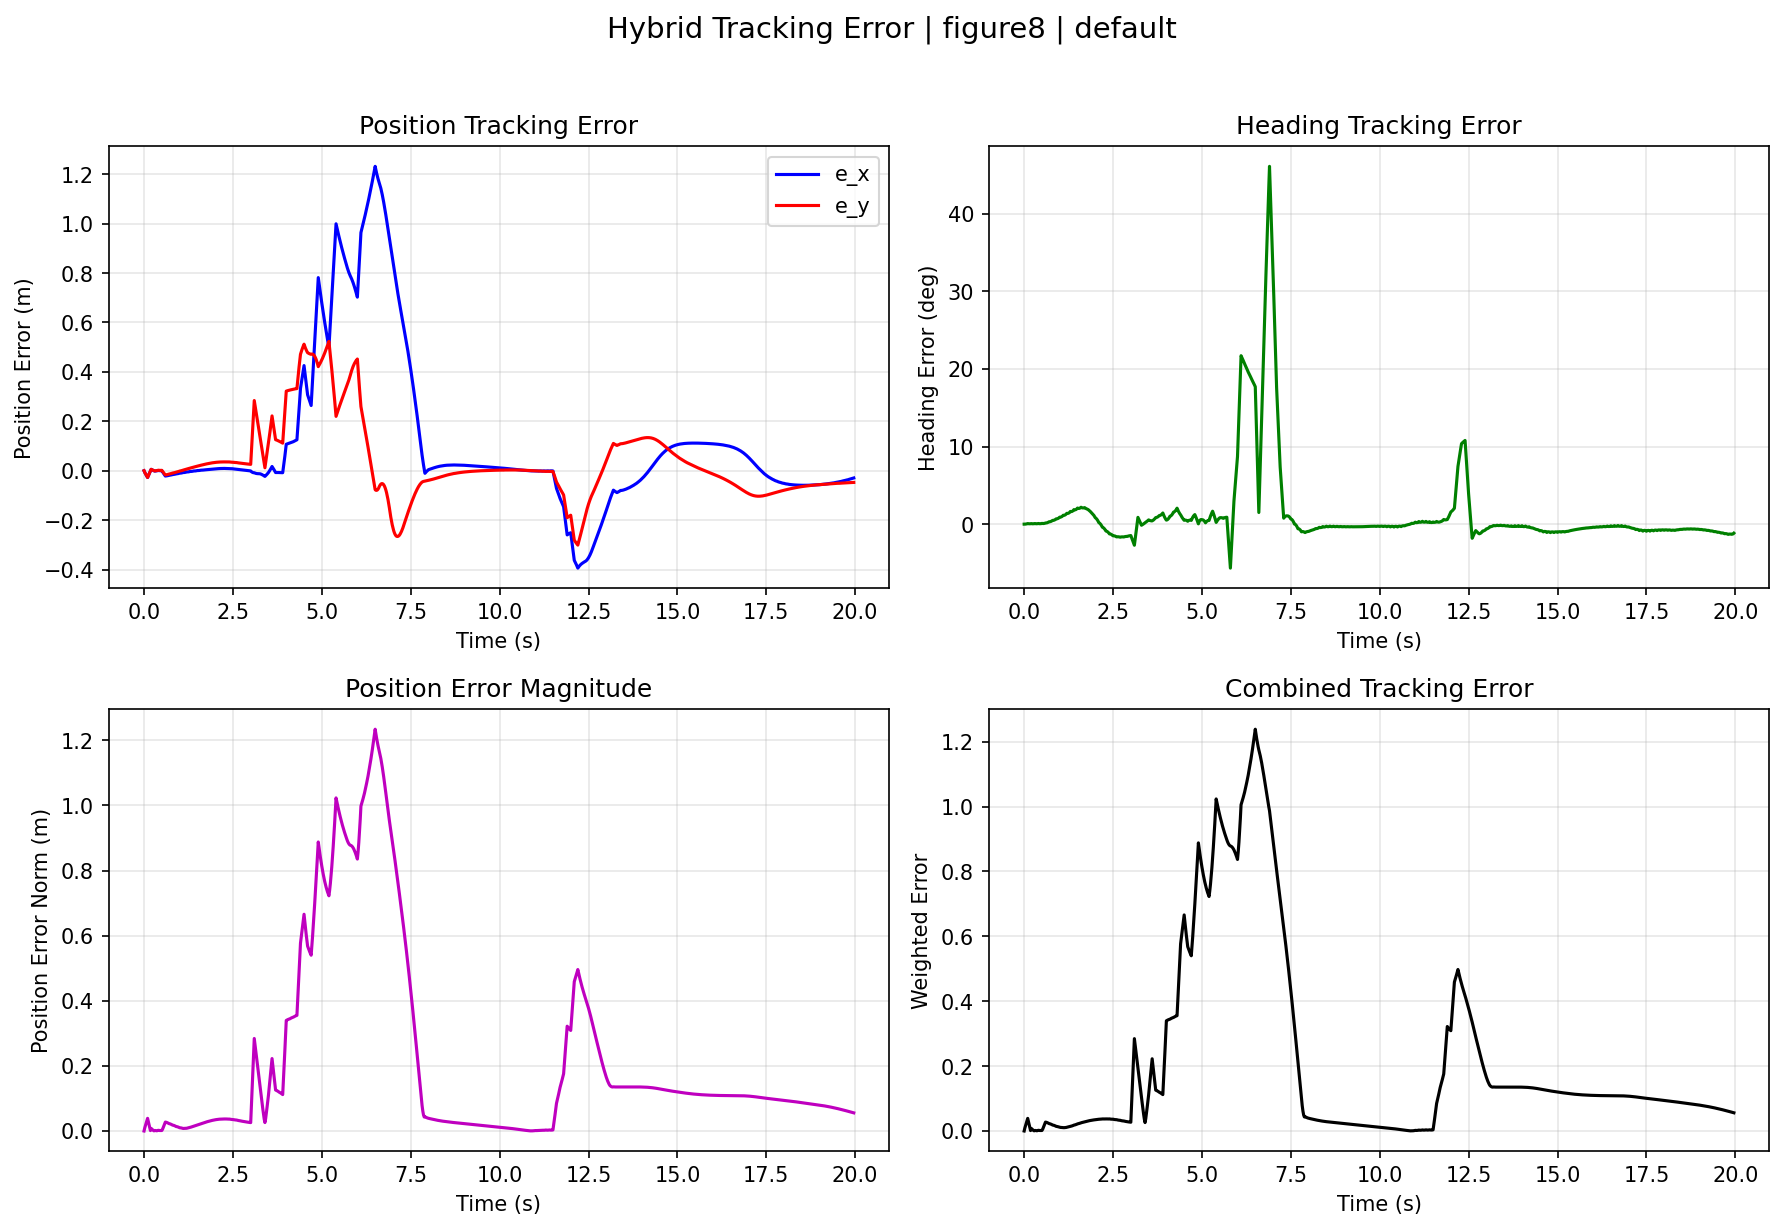
\includegraphics[width=0.85\textwidth]{hybrid_figure8_default_error.png}
    \caption{Hybrid tracking error over time. Error spikes correspond to obstacle avoidance maneuvers but quickly recover.}
    \label{fig:hybrid_error}
\end{figure}

\begin{figure}[H]
    \centering
    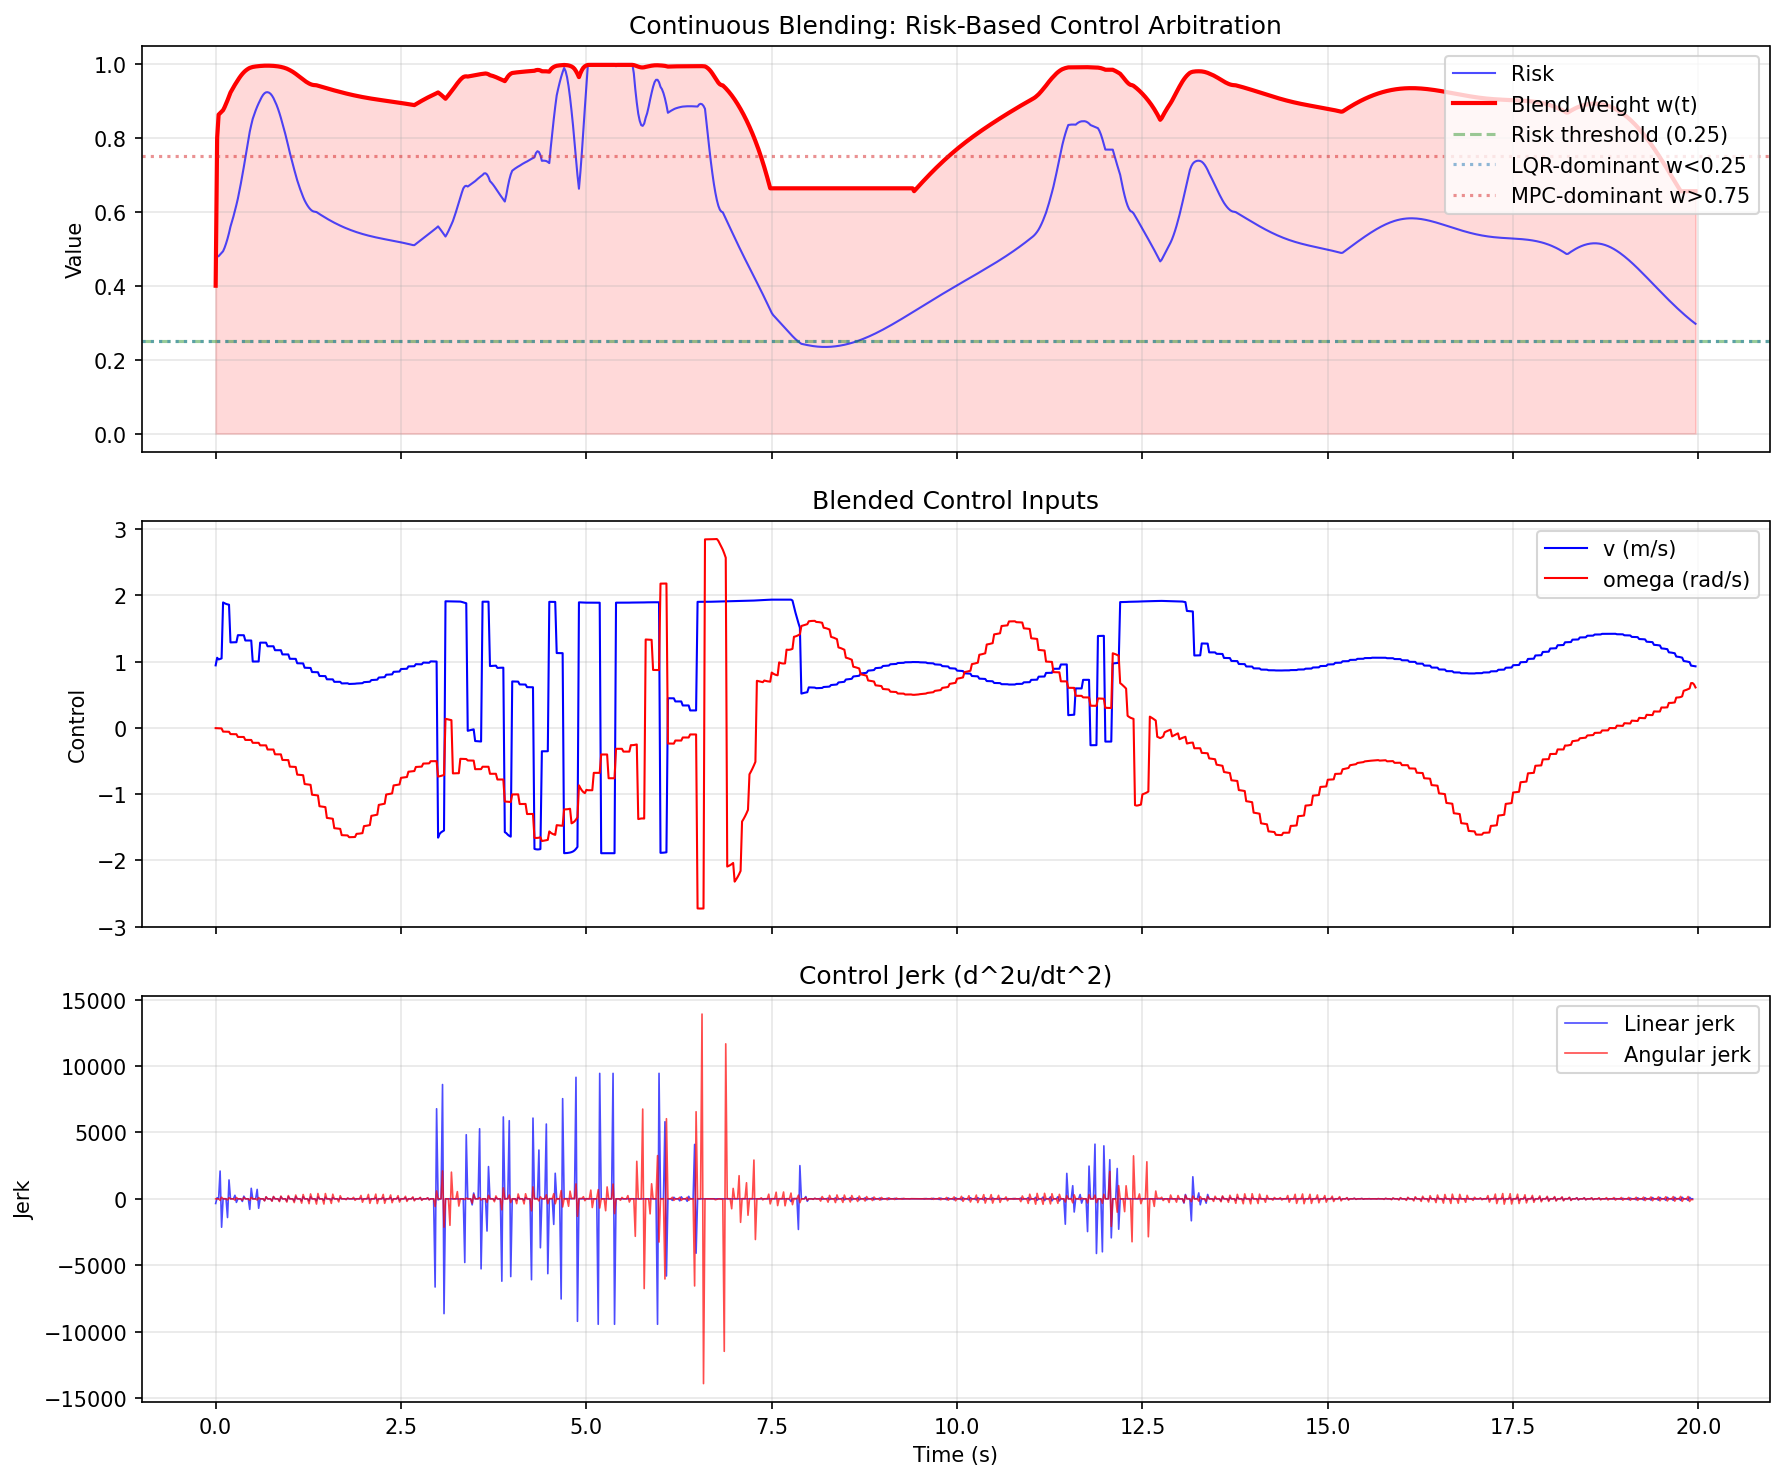
\includegraphics[width=0.85\textwidth]{hybrid_figure8_default_blending.png}
    \caption{Blending weight $w(t)$ and risk level over time. The sigmoid-based supervisor smoothly transitions between LQR-dominant and MPC-dominant modes.}
    \label{fig:hybrid_blending}
\end{figure}

\begin{figure}[H]
    \centering
    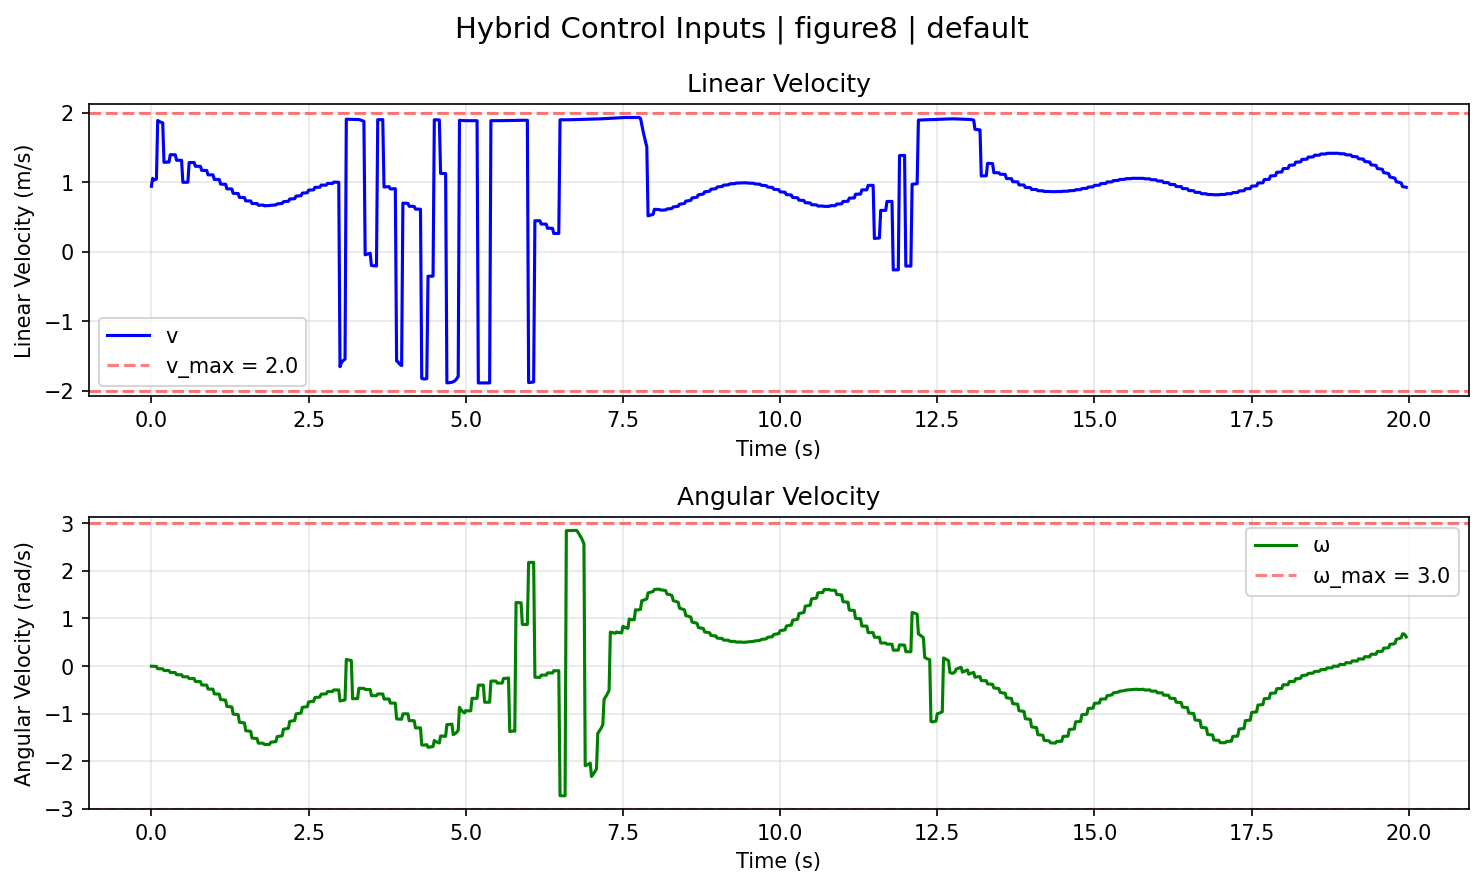
\includegraphics[width=0.85\textwidth]{hybrid_figure8_default_control.png}
    \caption{Hybrid control inputs showing smooth blending between LQR and MPC commands.}
    \label{fig:hybrid_control}
\end{figure}


%% ============================================================
\section{Comparative Summary}
%% ============================================================

\begin{table}[H]
\centering
\caption{Performance comparison across all four controllers on the figure-8 trajectory (20 seconds, $\Delta t = 0.02$s).}
\label{tab:comparison}
\begin{tabular}{@{}lcccc@{}}
\toprule
\textbf{Metric} & \textbf{LQR} & \textbf{Tube MPC} & \textbf{Adaptive NMPC} & \textbf{Hybrid} \\
\midrule
Mean Error (m)        & 0.005  & 1.638  & 1.282  & 0.218  \\
Final Error (m)       & 0.003  & 2.269  & 1.978  & 0.056  \\
Mean Solve Time (ms)  & $<$1   & 163    & 145    & 102    \\
Obstacles             & None   & 3      & 3      & 3      \\
Collisions            & N/A    & 163    & 355    & 0      \\
\bottomrule
\end{tabular}
\end{table}

\textbf{Key observations:}
\begin{itemize}
    \item LQR is the fastest and most accurate but has \emph{no} obstacle avoidance capability.
    \item Tube MPC provides obstacle awareness but the linearized constraints lead to conservative or sometimes insufficient avoidance (163 collision events).
    \item Adaptive NMPC achieves lower tracking error than Tube MPC due to exact nonlinear dynamics, but the more aggressive paths result in more near-misses (355 collisions).
    \item The Hybrid controller achieves the best of both worlds: near-LQR tracking accuracy in safe zones with effective obstacle avoidance, and zero recorded collisions in this scenario.
\end{itemize}


%% ============================================================
\section{Debugging Journey: Failures and Fixes}
%% ============================================================

This section honestly documents the critical failures we encountered and how we resolved them.

\subsection{Failure 1: Velocity Clipping Caused Robot Stalling}
\textbf{Problem:} All four controllers initially clipped the linear velocity to $v \in [0, v_{\max}]$, preventing any reverse motion. When the robot overshot a curve or needed to recover from a heading misalignment, the controller would command a negative $v$ to back up. Because this was clipped to zero, the robot stalled permanently while the reference trajectory moved on, causing exponentially growing tracking error.

\textbf{Fix:} We changed the clipping to $v \in [-v_{\max}, v_{\max}]$ across all controller nodes, allowing the differential-drive robot to reverse naturally. This single change resolved the stalling in LQR, MPC, and Hybrid modes.

\subsection{Failure 2: Hybrid Pure Pursuit Oscillation}
\textbf{Problem:} After dodging an obstacle, the Hybrid controller's pure-pursuit logic searched for a target waypoint at a distance of $0.4$m \emph{from the robot}. Since the robot was already pushed $>0.4$m away from the path, the algorithm selected the closest trajectory point, causing a harsh $90^\circ$ turn. The robot would overshoot the path, triggering the same behavior in reverse, resulting in back-and-forth wandering.

\textbf{Fix:} We changed the pure-pursuit search to find a point $0.4$m ahead \emph{along the trajectory} starting from the nearest path point. This guarantees a smooth, forward-facing merge regardless of the robot's cross-track deviation.

\subsection{Failure 3: MPC Cold-Start Infeasibility}
\textbf{Problem:} The CVXPY-based Tube MPC failed to find a solution on the first few timesteps if the initial heading error was large. The linearized obstacle constraints were immediately violated, and without slack variables the problem was infeasible. The robot would not move at all.

\textbf{Fix:} We enabled soft constraints with slack variables ($\rho = 5000$) by default, allowing the solver to always return a usable solution even when hard constraints cannot be exactly satisfied.

\subsection{Failure 4: RViz Reference Path Flickering}
\textbf{Problem:} In the ROS2 deployment, the reference trajectory displayed in RViz would appear and disappear randomly. We were publishing the static path at 1 Hz with a continuously updating timestamp, causing RViz to clear and redraw the path every second with network-induced jitter.

\textbf{Fix:} We switched the reference path publisher to use the \texttt{TRANSIENT\_LOCAL} QoS durability policy and published the path exactly once. The ROS middleware permanently stores the message, so any late-joining RViz subscriber immediately receives the complete path without flickering.

\subsection{Failure 5: BlendingSupervisor API Mismatch}
\textbf{Problem:} The \texttt{run\_simulation.py} script passed \texttt{lqr\_dominant\_threshold} and \texttt{mpc\_dominant\_threshold} as constructor keyword arguments to \texttt{BlendingSupervisor}, but the class only accepts them as internal attributes.

\textbf{Fix:} We removed the invalid kwargs from the constructor call and set the attributes directly on the instance after construction.


%% ============================================================
\section{ROS2 Implementation}
%% ============================================================

The complete framework was deployed as a ROS2 Jazzy package running inside a Docker container. This ensures reproducibility and isolates the complex dependency chain (CVXPY, CasADi, IPOPT, Gazebo).

\subsection{Architecture}
The ROS2 workspace contains two packages:
\begin{itemize}
    \item \texttt{hybrid\_controller}: A pure Python package containing the core control algorithms (LQR, MPC, Adaptive MPC, Hybrid Blender, Risk Metrics).
    \item \texttt{hybrid\_nav}: A ROS2 package containing the controller nodes, launch files, and RViz configuration for the Turtlebot3 Burger.
\end{itemize}

Each controller is wrapped as a ROS2 node that subscribes to \texttt{/odom} and \texttt{/obstacles}, computes the control output at 20 Hz, and publishes \texttt{TwistStamped} on \texttt{/cmd\_vel}. Additionally, each node publishes:
\begin{itemize}
    \item \texttt{/hybrid/reference\_path} (TRANSIENT\_LOCAL): The full reference trajectory for RViz.
    \item \texttt{/hybrid/robot\_trail}: A continuously growing \texttt{nav\_msgs/Path} for visualizing the robot's actual path.
    \item Diagnostic topics for tracking error, controller mode, and blending weight.
\end{itemize}

\subsection{Logging}
Every controller node writes a CSV-formatted telemetry log to \texttt{logs/} with columns: \texttt{Tick, X, Y, Theta, Error, V, Omega, Mode}. This enables post-run debugging of stalls, oscillations, and solver failures.

\subsection{Simulation Video}
A video demonstration of the ROS2 Gazebo simulation is available at:

\vspace{0.3cm}
\noindent\textbf{YouTube:} \url{https://youtube.com/placeholder-link}
\vspace{0.3cm}

\noindent\textit{(Link to be updated after video upload.)}


%% ============================================================
\section{What Remains and Future Scope}
%% ============================================================

\subsection{Current Limitations}
\begin{itemize}
    \item \textbf{Collision count in standalone MPC/AMPC:} The Tube MPC and Adaptive NMPC still record collision events in the offline simulation. The linearized obstacle constraints (MPC) and the aggressive nonlinear paths (AMPC) need further tuning of $d_{\text{safe}}$ and slack penalties.
    \item \textbf{Solver latency:} The mean MPC solve time of 100--160 ms is acceptable for 20 Hz control but would be insufficient for faster dynamics. Code-generated solvers (e.g., via \texttt{cvxpygen}) were partially implemented but not deployed.
    \item \textbf{Dynamic obstacles:} The current framework treats obstacles as static. Obstacle velocity estimation and predictive avoidance are not implemented.
\end{itemize}

\subsection{Future Work}
\begin{enumerate}
    \item \textbf{Hardware deployment:} Port the Dockerized ROS2 nodes to a physical Turtlebot3 and replace pseudo-obstacles with real LiDAR-based clustering.
    \item \textbf{Dynamic obstacle prediction:} Integrate a Kalman filter or constant-velocity model to predict obstacle trajectories, extending the MPC constraints into spatiotemporal tubes.
    \item \textbf{C++ code generation:} Use CasADi's C code generation to achieve $>50$ Hz control rates on embedded hardware.
    \item \textbf{Multi-agent extension:} Extend the framework to multi-robot coordination with inter-robot collision avoidance.
    \item \textbf{Formal safety guarantees:} Integrate Control Barrier Functions (CBFs) to provide provable safety certificates alongside the MPC constraints.
\end{enumerate}


%% ============================================================
\section*{References}
%% ============================================================

\begin{enumerate}[label={[\arabic*]}]
    \item B.\ Anderson and J.\ Moore, \textit{Optimal Control: Linear Quadratic Methods}, Dover Publications, 2007.
    \item J.\ Rawlings, D.\ Mayne, and M.\ Diehl, \textit{Model Predictive Control: Theory, Computation, and Design}, 2nd ed., Nob Hill Publishing, 2017.
    \item J.\ K\"ohler et al., ``Certainty-Equivalent Adaptive MPC for Uncertain Nonlinear Systems,'' in \textit{Proc.\ IEEE CDC}, 2026.
    \item J.\ A.\ E.\ Andersson et al., ``CasADi: A Software Framework for Nonlinear Optimization and Optimal Control,'' \textit{Mathematical Programming Computation}, vol.\ 11, pp.\ 1--36, 2019.
    \item S.\ Diamond and S.\ Boyd, ``CVXPY: A Python-Embedded Modeling Language for Convex Optimization,'' \textit{Journal of Machine Learning Research}, vol.\ 17, no.\ 83, pp.\ 1--5, 2016.
    \item ROBOTIS, ``TurtleBot3 e-Manual,'' \url{https://emanual.robotis.com/docs/en/platform/turtlebot3/overview/}.
    \item Open Robotics, ``ROS 2 Jazzy Jalisco Documentation,'' \url{https://docs.ros.org/en/jazzy/}.
\end{enumerate}

\end{document}
